%==============================================================
\chapter{DESIGN SPECIFICATIONS}
\label{ch:design}
%==============================================================

\tikzset{
  blk/.style={draw, rounded corners=2pt, align=center, inner sep=2.5pt, fill=white, font=\scriptsize},
  dblk/.style={blk, fill=sxlight},
  hblk/.style={blk, fill=sxhead, font=\scriptsize\bfseries},
  arr/.style={-{Stealth[length=1.8mm]}, thick},
  darr/.style={-{Stealth[length=1.8mm]}, thick, dashed},
  grp/.style={draw, rounded corners=4pt, inner sep=4pt},
  actor/.style={draw, circle, minimum size=4mm, inner sep=0pt},
}

\section{System Architecture}
\label{sec:arch}

\figref{fig:arch} shows the architecture of the complete product. The device is one Python process (on the Pi, a systemd user service with a watchdog) that owns the camera, the pipeline, the Local Console, the SOS engine, the channels and the link. The pipeline is split into threads so that slow inference never blocks the video: a \emph{capture} thread reads every frame at the camera rate into a newest-frame slot; an \emph{inference} thread takes the newest frame (tick mode, at most 6\,Hz) or the newest 4\,s clip (clip mode, every 2\,s); face recognition runs on its own \emph{identity} thread; the \emph{audio} engine reads the microphone continuously; and the \emph{preview} composites every captured frame with the latest overlay, encoding it once for all viewers. Decisions flow from perception through evidence, TCI and level policy to incidents and side effects, and an idempotent trigger hands alarm-class incidents to the SOS engine. The device opens only outbound connections; the Portal reaches it through the link.

\begin{figure}[htbp]
\centering
\resizebox{\textwidth}{!}{%
\begin{tikzpicture}[node distance=2.5mm]
% inputs
\node[dblk, text width=1.75cm] (cam) at (0,0) {Camera\\(Pi CSI, USB,\\RTSP, file)};
\node[dblk, text width=1.75cm, below=5mm of cam] (mic) {USB\\microphone};
\node[dblk, text width=1.75cm, below=5mm of mic] (gpioin) {PIR, door,\\mains sense};
% device column 1
\node[blk, text width=2.3cm, right=6mm of cam] (cap) {Capture thread\\newest-frame slot};
\node[blk, text width=2.3cm, below=of cap] (inf) {Inference: tick\\(6\,Hz) or 4\,s clip};
\node[blk, text width=2.3cm, below=of inf] (perc) {Perception: YOLO,\\DINOv2, faces, OSNet,\\PANNs, motion};
\node[blk, text width=2.3cm, below=of perc] (ev) {Evidence rules\\($k$-of-$n$, gates,\\modalities)};
% device column 2
\node[blk, text width=2.3cm, right=3mm of cap] (prev) {Preview + HUD\\MJPEG for viewers};
\node[blk, text width=2.3cm, below=of prev] (tci) {TCI engine and\\level policy};
\node[blk, text width=2.3cm, below=of tci] (inc) {Incidents, event log,\\evidence vault};
\node[blk, text width=2.3cm, below=of inc] (sos) {SOS engine, sweeper,\\PINs, policy};
% device column 3
\node[blk, text width=2.15cm, right=3mm of prev] (lc) {Local Console\\(FastAPI + React)};
\node[blk, text width=2.15cm, below=of lc] (hw) {GPIO: siren relay,\\LEDs; node watchdog};
\node[blk, text width=2.15cm, below=of hw] (ch) {Channels + outbox\\behind send guard};
\node[blk, text width=2.15cm, below=of ch] (link) {Link client:\\outbox, tunnel,\\video relay};
\begin{scope}[on background layer]
\node[grp, fill=sxhead!35, fit=(cap)(ev)(lc)(link), label={[font=\scriptsize\bfseries]above:Device (Raspberry Pi 5): python -m sentrix}] (dev) {};
\end{scope}
% portal
\node[blk, text width=2.15cm, below=12mm of link] (hub) {Link hub + tunnel\\proxy /d/\{device\}/};
\node[blk, text width=2.3cm, left=3mm of hub] (csos) {SOS mirror, cloud\\authority, Desk};
\node[blk, text width=2.3cm, left=3mm of csos] (acct) {Accounts, onboarding,\\household, admin};
\node[blk, text width=2.15cm, below=of hub] (notify) {Notification worker:\\Telegram, e-mail};
\node[blk, text width=2.3cm, left=3mm of notify] (spa) {Portal React app,\\JSON API v2};
\node[blk, text width=2.3cm, left=3mm of spa] (db) {SQLite (1\,GB disk),\\audit hash chain};
\begin{scope}[on background layer]
\node[grp, fill=sxlight!60, fit=(hub)(csos)(acct)(notify)(db)(spa), label={[font=\scriptsize\bfseries]below:Portal (Render, Docker): python -m sentrix\_portal}] (por) {};
\end{scope}
\draw[arr] (cam) -- (cap);
\draw[arr] (mic.east) -- ++(2mm,0) |- (perc.west);
\draw[arr] (gpioin.east) -- ++(4mm,0) |- (ev.west);
\draw[arr] (cap) -- (inf);
\draw[arr] (inf) -- (perc);
\draw[arr] (perc) -- (ev);
\draw[arr] (cap) -- (prev);
\draw[arr] (ev.east) -- ++(1.5mm,0) |- (tci.west);
\draw[arr] (tci) -- (inc);
\draw[arr] (inc) -- (sos);
\draw[arr] (prev) -- (lc);
\draw[arr] (tci.east) -- (hw.west);
\draw[arr] (sos.east) -- (ch.west);
\draw[arr] (sos.east) ++(0,-1mm) -- (link.west);
\draw[arr, <->] (link.south) -- node[right, font=\tiny, align=left]{WSS link,\\outbound only} (hub.north);
\end{tikzpicture}}
\caption{System architecture of SENTRIX: device threads and services, and the Portal}
\label{fig:arch}
\end{figure}

\paragraph{Component view.} \figref{fig:components} groups the code into packages and shows their dependencies. The device package is layered: \code{io} and \code{perception} know nothing of alarms; \code{fusion} turns votes into evidence and levels; \code{pipeline} orchestrates; \code{sos}, \code{alerting} and \code{link} act on decisions; \code{web} exposes everything to the two React applications. The Portal shares the send guard, the SOS state table and the link protocol with the device, so both sides apply the same rules.

\begin{figure}[htbp]
\centering
\resizebox{\textwidth}{!}{%
\begin{tikzpicture}[node distance=3mm,
  pkg/.style={draw, fill=sxlight, align=left, font=\tiny, text width=2.55cm, inner sep=2pt, rounded corners=1pt},
  title/.style={font=\scriptsize\bfseries}]
\node[pkg] (io) at (0,0) {\textbf{io}\\cameras, demo reel, Picamera2, siren, GPIO, node, recorder, Wi-Fi};
\node[pkg, right=of io] (perc) {\textbf{perception}\\detector, scene, identity, OSNet re-id, audio + sound tagger, motion};
\node[pkg, right=of perc] (fus) {\textbf{fusion}\\evidence, TCI, level policy, calibration};
\node[pkg, right=of fus] (runtime) {\textbf{runtime}\\torch / ONNX / NCNN backends};
\node[pkg, below=5mm of perc] (pipe) {\textbf{pipeline}\\engine (tick), clip engine, fast lane, incidents, events, state};
\node[pkg, left=of pipe] (evid) {\textbf{evidence, storage}\\AES-GCM vault, SQLite};
\node[pkg, right=of pipe] (sos) {\textbf{sos}\\states, machine, policy, PINs, sweeper, service};
\node[pkg, right=of sos] (alert) {\textbf{alerting}\\send guard, router, outbox, Telegram, e-mail, modem};
\node[pkg, below=5mm of pipe] (web) {\textbf{web}\\Local Console API, auth, CSP/CSRF, recording routes};
\node[pkg, right=of web] (link) {\textbf{link}\\client, protocol, tunnel, path table, commands};
\node[pkg, below=9mm of web, xshift=-1.6cm] (fe) {\textbf{frontend} (TypeScript)\\React device app + Portal app, ui, api packages};
\node[pkg, below=9mm of link, xshift=1.6cm] (portal) {\textbf{sentrix\_portal} (cloud)\\routes, services (hub, SOS, notify, retention); shares guard, SOS states, link protocol};
\begin{scope}[on background layer]
\node[draw, dashed, rounded corners=3pt, fit=(io)(runtime)(evid)(alert)(web)(link), inner sep=3pt, label={[font=\scriptsize\itshape]above:package sentrix (device)}] {};
\end{scope}
\draw[darr] (pipe) -- (perc); \draw[darr] (pipe) -- (fus); \draw[darr] (pipe.north west) -- (io.south east);
\draw[darr] (perc) -- (io); \draw[darr] (perc.north east) to[bend left=12] (runtime.north west);
\draw[darr] (pipe) -- (evid); \draw[darr] (pipe) -- (sos); \draw[darr] (sos) -- (alert);
\draw[darr] (web) -- (pipe); \draw[darr] (web) -- (link); \draw[darr] (fe) -- (web);
\draw[darr] (link) -- (sos); \draw[darr] (portal) -- (link);
\end{tikzpicture}}
\caption{Component (package) diagram; dashed arrows point from a package to the packages it uses}
\label{fig:components}
\end{figure}

%--------------------------------------------------------------
\section{Design Level Diagrams}
\label{sec:diagrams}

\subsection{Use Case Diagram}
\figref{fig:usecase} shows the actors and their main use cases. The device itself is an actor for the use cases it starts on its own (raising an alarm, prompting the owner).

\begin{figure}[htbp]
\centering
\begin{tikzpicture}[uc/.style={draw, ellipse, align=center, font=\tiny, inner sep=1pt, minimum height=6.5mm, text width=2.35cm, fill=sxlight},
  act/.style={align=center, font=\scriptsize}]
\newcommand{\stick}[2]{\node[act] (#1) at #2 {\tikz{\draw (0,0.32) circle (0.09); \draw (0,0.23)--(0,0.04) (-0.13,0.16)--(0.13,0.16) (0,0.04)--(-0.1,-0.1) (0,0.04)--(0.1,-0.1);}};}
% use cases (two columns)
\foreach \n/\t/\x/\y in {u1/{Activate account and onboard}/3.4/6.2, u2/{Watch live view and level}/3.4/5.4, u3/{Answer an alert (approve, PIN, checking)}/3.4/4.6, u4/{Manage contacts and settings}/3.4/3.8, u5/{Export or erase data}/3.4/3.0, u6/{Confirm consent, see alert page}/3.4/2.2, u7/{Acknowledge and close request}/3.4/1.4,
  u8/{Raise alarm and seal evidence}/7.0/6.2, u9/{Prompt owner, alert contacts}/7.0/5.4, u10/{Sound siren, show LEDs}/7.0/4.6, u11/{Enrol faces}/7.0/3.8, u12/{Record training video}/7.0/3.0, u13/{Provision device, create customer}/7.0/2.2, u14/{Review audit log}/7.0/1.4}
  {\node[uc] (\n) at (\x,\y) {\t};}
\node[draw, thick, rounded corners=3pt, fit=(u1)(u8)(u7)(u14), inner sep=5pt, label={[font=\scriptsize\bfseries]above:SENTRIX}] (sys) {};
\stick{owner}{(0,5.6)} \node[act, below=-1mm of owner] {Owner /\\member};
\stick{contact}{(0,3.4)} \node[act, below=-1mm of contact] {Emergency\\contact};
\stick{desk}{(0,1.4)} \node[act, below=-1mm of desk] {Desk\\operator};
\stick{dev}{(10.4,5.6)} \node[act, below=-1mm of dev] {SENTRIX\\device};
\stick{dadmin}{(10.4,3.4)} \node[act, below=-1mm of dadmin] {Device\\admin};
\stick{cadmin}{(10.4,1.6)} \node[act, below=-1mm of cadmin] {Company\\admin};
\foreach \u in {u1,u2,u3,u4,u5} \draw (owner) -- (\u.west);
\draw (contact) -- (u6.west);
\draw (desk) -- (u7.west);
\foreach \u in {u8,u9,u10} \draw (dev) -- (\u.east);
\draw (dadmin) -- (u11.east); \draw (dadmin) -- (u12.east);
\draw (cadmin) -- (u13.east); \draw (cadmin) -- (u14.east);
\end{tikzpicture}
\caption{Use case diagram}
\label{fig:usecase}
\end{figure}

\subsection{Class Diagram}
\figref{fig:class} shows the main classes of the device's decision path and their associations (methods abridged).

\begin{figure}[htbp]
\centering
\resizebox{0.92\textwidth}{!}{%
\begin{tikzpicture}[
  cls/.style={draw, rectangle split, rectangle split parts=2, align=left, font=\tiny, fill=white, rectangle split part fill={sxhead,white}, text width=2.75cm, inner sep=1.5pt},
  note/.style={font=\tiny\itshape},
  comp/.style={-{Diamond[open]}}, use/.style={-{Stealth[length=1.6mm]}}]
% column x: 0 (perception), 3.9 (decision chain), 7.8 (outputs)
\node[cls] (src)   at (0,0)    {\textbf{FrameSource}\nodepart{second}+read() / latest()\\{\itshape Capture, PiCamera, DemoReel}};
\node[cls] (pipe)  at (3.9,0)  {\textbf{Pipeline}\nodepart{second}+observe(frame, t)\\+decide(obs)\\+process(frame, t)\\+run\_live()};
\node[cls] (clip)  at (7.8,0)  {\textbf{ClipEngine}\nodepart{second}+analyse(clip)\\{\itshape ClipBuffer, FastLane}};
\node[cls] (det)   at (0,-1.7) {\textbf{Detector}\nodepart{second}+detect(frame)\\+reset\_tracks()};
\node[cls] (scene) at (0,-3.0) {\textbf{SceneEngine}\nodepart{second}+score\_frames(frames)\\+decide(probs)};
\node[cls] (ident) at (0,-4.3) {\textbf{TrackIdentity}\nodepart{second}+update(tracks, faces, bodies)\\{\itshape IdentityWorker, ReIDEngine}};
\node[cls] (audio) at (0,-5.6) {\textbf{AudioEngine}\nodepart{second}+classify\_window()\\+result\_for(t)};
\node[cls] (evid)  at (3.9,-1.9) {\textbf{EvidenceAccumulator}\nodepart{second}+update(sources, context)\\{\itshape ConfirmationWindow, Vote}};
\node[cls] (tci)   at (3.9,-3.2) {\textbf{TCIEngine}\nodepart{second}+compute(features) $\rightarrow$ TCIResult};
\node[cls] (pol)   at (3.9,-4.3) {\textbf{LevelPolicy}\nodepart{second}+update(tci, t)\\+level};
\node[cls] (inc)   at (3.9,-5.6) {\textbf{IncidentManager}\nodepart{second}+update(result)\\+claim(side effect)\\{\itshape PeakSnapshot}};
\node[cls] (vault) at (7.8,-1.9) {\textbf{EvidenceVault}\nodepart{second}+save(frame, meta)\\+verify\_chain()};
\node[cls] (log)   at (7.8,-3.2) {\textbf{EventLog}\nodepart{second}+write(row)\\+audit(event)};
\node[cls] (sos)   at (7.8,-5.6) {\textbf{SosEngine}\nodepart{second}+trigger(incident)\\+respond(action, PIN)\\+sweep(now)};
\node[cls] (router) at (7.8,-7.1) {\textbf{Router}\nodepart{second}+send(message)\\{\itshape send guard, outbox}};
\node[cls] (link)  at (3.9,-7.1) {\textbf{LinkService}\nodepart{second}+start() / stop()\\+is\_online};
% perception bus into the pipeline
\foreach \c/\y in {det/-1.7,scene/-3.0,ident/-4.3,audio/-5.6} \draw (\c.east) -- (1.75,\y);
\draw (1.75,-5.6) -- (1.75,-0.25);
\draw[comp] (1.75,-0.25) -- ([yshift=-2.5mm]pipe.west);
\draw[comp] ([yshift=2.5mm]src.east) -- ([yshift=2.5mm]pipe.west);
\draw[comp] (clip.west) -- (pipe.east);
\draw[comp] (evid.north) -- (pipe.south);
\draw[use] (evid) -- (tci); \draw[use] (tci) -- (pol); \draw[use] (pol) -- (inc);
\draw[use] (pipe.south east) -- (vault.north west);
\draw[use] (vault) -- (log);
\draw[use] (inc.east) -- (sos.west);
\draw[use] (sos) -- (router);
\draw[use] (router.west) -- (link.east);
\draw[use] (inc.south) -- node[left, note]{events} (link.north);
\end{tikzpicture}}
\caption{Class diagram of the decision path (diamond: composition, arrow: uses)}
\label{fig:class}
\end{figure}

\subsection{Sequence Diagram}
\figref{fig:sequence} follows a confirmed handgun from the camera to a closed request, in the order the components act.

\begin{figure}[htbp]
\centering
\begin{tikzpicture}[font=\tiny, ll/.style={draw, fill=sxhead, font=\scriptsize\bfseries, minimum width=1.6cm, align=center},
  msg/.style={-{Stealth[length=1.5mm]}}, ret/.style={-{Stealth[length=1.5mm]}, dashed}]
\foreach \i/\n/\x in {1/Camera/0, 2/Pipeline/2.05, 3/{Evidence,\\TCI, policy}/4.1, 4/{SOS engine}/6.15, 5/Portal/8.2, 6/Owner/10.25, 7/{Contacts,\\Desk}/12.3}
  {\node[ll] (h\i) at (\x,0) {\n}; \draw[gray] (h\i.south) -- (\x,-10.4);}
\newcommand{\m}[4]{\draw[msg] (#1,#3) -- node[above, align=center, fill=white, inner sep=1pt]{#4} (#2,#3);}
\newcommand{\rr}[4]{\draw[ret] (#1,#3) -- node[above, align=center, fill=white, inner sep=1pt]{#4} (#2,#3);}
\m{0}{2.05}{-0.8}{frames (15--30 fps)}
\m{2.05}{4.1}{-1.4}{votes: detector, scene,\\aligned audio}
\draw[msg] (4.1,-1.9) -- ++(0.35,0) |- node[right, pos=0.25, align=left]{2 of 3 fresh\\confirmations} (4.1,-2.5);
\rr{4.1}{2.05}{-3.0}{Level 3 committed}
\draw[msg] (2.05,-3.3) -- ++(0.35,0) |- node[right, pos=0.25, align=left]{snapshot,\\AES-GCM bundle} (2.05,-3.9);
\m{2.05}{6.15}{-4.4}{trigger(incident) (idempotent)}
\m{6.15}{8.2}{-4.9}{request PENDING\\over the link}
\m{8.2}{10.25}{-5.5}{``Do you need assistance?''\\Portal, Telegram, e-mail}
\rr{10.25}{8.2}{-6.3}{approve (Police)}
\m{8.2}{6.15}{-6.9}{answer relayed}
\rr{6.15}{8.2}{-7.5}{APPROVED $\rightarrow$ dispatch package}
\m{8.2}{12.3}{-8.1}{alert + snapshot, address, timeline}
\rr{12.3}{8.2}{-8.8}{Desk: acknowledge}
\m{8.2}{10.25}{-9.3}{``The Desk is handling it''}
\rr{12.3}{8.2}{-10.0}{resolve (outcome) $\rightarrow$ CLOSED, verdict TRUE}
\end{tikzpicture}
\caption{Sequence diagram: from a confirmed handgun to a closed assistance request}
\label{fig:sequence}
\end{figure}

\subsection{State Machine Diagram}
The assistance request is the most safety-critical object in the product; its states and transitions (\figref{fig:sosstates}) are a fixed table in \code{sentrix/sos/states.py} shared by the device and the Portal. Terminal states are Closed, Declined, Expired and Cancelled; Closed can only be reached along the help path, so a request is never ``closed'' without someone having been asked to help.

\begin{figure}[htbp]
\centering
\resizebox{\textwidth}{!}{%
\begin{tikzpicture}[st/.style={draw, rounded corners=6pt, fill=sxlight, font=\scriptsize\bfseries, minimum width=2.1cm, minimum height=7mm, align=center},
  term/.style={st, fill=sxhead, double},
  tr/.style={-{Stealth[length=1.8mm]}, thick}, lab/.style={font=\tiny, align=center, fill=white, inner sep=1pt}]
\node[circle, fill=black, inner sep=2pt] (init) at (-2.0,0) {};
\node[st] (dr) at (0,0) {DRAFTED};
\node[st] (pe) at (3.0,0) {PENDING};
\node[st] (ap) at (6.6,0) {APPROVED};
\node[st] (di) at (10.4,0) {DISPATCHED};
\node[st] (fa) at (6.6,-2.6) {FAILED};
\node[st] (ac) at (10.4,-2.6) {ACKNOWLEDGED};
\node[term] (cl) at (8.5,-5.0) {CLOSED};
\node[term] (de) at (-0.6,-3.6) {DECLINED};
\node[term] (ca) at (1.5,-3.6) {CANCELLED};
\node[term] (ex) at (3.6,-3.6) {EXPIRED};
\node[draw, dashed, rounded corners=5pt, fit=(dr)(pe), inner sep=7pt, label={[font=\tiny\itshape]above left:Prompting (owner asked)}] (prompt) {};
\node[draw, dashed, rounded corners=5pt, fit=(ap)(di)(fa)(ac), inner sep=7pt, label={[font=\tiny\itshape]above right:Help path}] (help) {};
\draw[tr] (init) -- node[lab, above]{created} (dr);
\draw[tr] (dr) -- node[lab, above]{prompted} (pe);
\draw[tr] (pe) -- node[lab, above]{approve / duress PIN} (ap);
\draw[tr] (dr.north) to[out=40, in=140] node[lab, above]{approve (before the prompt)} (ap.north);
\draw[tr] (ap) -- node[lab, above]{delivered} (di);
\draw[tr] (ap) -- node[lab, left]{delivery\\failed} (fa);
\draw[tr] (fa.north east) -- node[lab, sloped, above, pos=0.55]{delivered} (di.south west);
\draw[tr] (fa.west) to[out=150, in=210] node[lab, left]{retry} (ap.west);
\draw[tr] (di) -- node[lab, right]{acknowledge} (ac);
\draw[tr] (fa) -- node[lab, below]{acknowledge} (ac);
\draw[tr] (ac.south) |- node[lab, pos=0.25, right]{resolve / stale close (24\,h)} (cl.east);
\draw[tr] (di.east) -- ++(5mm,0) |- (cl.east);
\draw[tr] (fa.south) |- node[lab, pos=0.3, left]{resolve / stale close} (cl.west);
\draw[tr] (prompt.south -| de) -- node[lab, left]{decline\\(SOS PIN)} (de);
\draw[tr] (prompt.south -| ca) -- node[lab, right]{cancel (FALSE\\verdict, reset)} (ca);
\draw[tr] (prompt.south -| ex) -- node[lab, right]{expire\\(window)} (ex);
\end{tikzpicture}}
\caption{State machine of an assistance request (double border: terminal states). Arrows leaving the Prompting box apply to both of its states; ``acknowledge'' is also accepted directly in Approved. Self-events such as reminders, ``I'm checking'', a level rise or the device going offline do not change the state.}
\label{fig:sosstates}
\end{figure}

\subsection{Activity Diagram}
\figref{fig:activity} shows one decision of the tick pipeline (the clip pipeline follows the same path with clip-level confirmation, \tabref{tab:clip}).

\begin{figure}[htbp]
\centering
\begin{tikzpicture}[node distance=3.2mm, act/.style={draw, rounded corners=5pt, fill=sxlight, font=\scriptsize, align=center, text width=4.2cm, minimum height=6mm},
  dec/.style={draw, diamond, aspect=2.6, fill=sxhead, font=\tiny, align=center, inner sep=0.5pt}, tr/.style={-{Stealth[length=1.6mm]}, thick}]
\node[circle, fill=black, inner sep=2.2pt] (s) at (0,0) {};
\node[act, below=of s] (a1) {Take the newest frame (drop older ones)};
\node[act, below=of a1] (a2) {Detect persons (tracks), weapons, fire};
\node[act, below=of a2] (a3) {Scene probabilities; latest face verdict per track; aligned audio window, if any};
\node[act, below=of a3] (a4) {Push fresh votes into each source's confirmation window};
\node[dec, below=of a4] (d1) {confirmed?};
\node[act, below=5mm of d1] (a5) {Score class: one modality (L3 band), two (L4--L5), three ($\geq$ L5)};
\node[act, right=14mm of d1, text width=3.0cm] (a5b) {Score below L2 (shown, not acted on)};
\node[act, below=of a5] (a6) {TCI = max(class evidence, unknown-person L2)};
\node[act, below=of a6] (a7) {Level policy: commit L2/L3 now; L4/L5 after 0.6\,s and 2 observations};
\node[dec, below=of a7] (d2) {level\\$\geq 3$?};
\node[act, below=5mm of d2] (a8) {Snapshot, evidence bundle; SOS trigger for alarm classes; L5: siren};
\node[act, right=14mm of d2, text width=3.0cm] (a8b) {Update incident, event log, dashboard};
\node[circle, draw, inner sep=2.2pt, below=of a8] (e) {}; \fill (e) circle (1.3pt);
\foreach \x/\y in {s/a1,a1/a2,a2/a3,a3/a4,a4/d1,a5/a6,a6/a7,a7/d2,a8/e} \draw[tr] (\x) -- (\y);
\draw[tr] (d1) -- node[right, font=\tiny]{yes} (a5);
\draw[tr] (d1) -- node[above, font=\tiny]{no} (a5b);
\draw[tr] (a5b.south) |- (a6.east);
\draw[tr] (d2) -- node[right, font=\tiny]{yes} (a8);
\draw[tr] (d2) -- node[above, font=\tiny]{no} (a8b);
\draw[tr] (a8b.south) |- (e.east);
\end{tikzpicture}
\caption{Activity diagram of one tick of the decision pipeline}
\label{fig:activity}
\end{figure}

\subsection{Data Flow Diagrams}
\figref{fig:dfd0} is the context (Level~0) diagram and \figref{fig:dfd1} the Level~1 diagram of the device's processes and data stores.

\begin{figure}[htbp]
\centering
\begin{tikzpicture}[ext/.style={draw, fill=sxhead, font=\scriptsize, align=center, minimum width=2.2cm, minimum height=7mm},
  proc/.style={draw, circle, fill=sxlight, font=\scriptsize\bfseries, align=center, minimum size=2.2cm}, fl/.style={-{Stealth[length=1.6mm]}, thick}, lab/.style={font=\tiny, align=center}]
\node[proc] (p) at (0,0) {0\\SENTRIX};
\node[ext] (room) at (-5,1.3) {Room\\(camera, mic, sensors)};
\node[ext] (owner) at (5,1.3) {Owner / member};
\node[ext] (cont) at (5,-1.3) {Contacts, Desk};
\node[ext] (adm) at (-5,-1.3) {Company admin,\\device admin};
\node[ext] (msg) at (0,-2.7) {Telegram, e-mail, SMS};
\draw[fl] (room) -- node[above, lab, sloped]{video, audio, events} (p);
\draw[fl] (p.north east) to[bend left=10] node[above, lab, sloped]{alerts, live view, incidents} (owner.west);
\draw[fl] (owner.south west) to[bend left=10] node[below, lab, sloped]{answers, PINs, settings} (p.east);
\draw[fl] (p) -- node[below, lab, sloped]{dispatch package} (cont);
\draw[fl] (cont.north west) to[bend right=25] node[above, lab, sloped, pos=0.6]{acknowledge, resolve} (p.east);
\draw[fl] (adm) -- node[below, lab, sloped]{provisioning, faces} (p);
\draw[fl] (p) -- node[right, lab]{messages (guarded)} (msg);
\end{tikzpicture}
\caption{Data flow diagram, Level 0 (context)}
\label{fig:dfd0}
\end{figure}

\begin{figure}[htbp]
\centering
\begin{tikzpicture}[proc/.style={draw, circle, fill=sxlight, font=\tiny, align=center, minimum size=1.55cm, inner sep=0pt},
  store/.style={draw, fill=white, font=\tiny, align=center, minimum width=2.1cm, minimum height=5mm, path picture={\draw ([xshift=3mm]path picture bounding box.north west) -- ([xshift=3mm]path picture bounding box.south west);}},
  ext/.style={draw, fill=sxhead, font=\tiny, align=center, minimum width=1.6cm, minimum height=6mm},
  fl/.style={-{Stealth[length=1.5mm]}, thick}, lab/.style={font=\tiny, align=center}]
\node[ext] (room) at (-6.4,0) {Room};
\node[proc] (p1) at (-4.2,0) {1.0\\Capture};
\node[proc] (p2) at (-1.6,0) {2.0\\Perceive};
\node[proc] (p3) at (1.0,0) {3.0\\Confirm and\\fuse};
\node[proc] (p4) at (3.6,0) {4.0\\Commit level,\\incident};
\node[proc] (p5) at (3.6,-3.0) {5.0\\Assistance\\request};
\node[proc] (p6) at (0.4,-3.0) {6.0\\Send\\(guarded)};
\node[proc] (p7) at (-3.0,-3.0) {7.0\\Link and\\tunnel};
\node[store] (d1) at (-1.6,1.8) {D1 Face gallery};
\node[store] (d2) at (3.6,1.8) {D2 Event log};
\node[store] (d3) at (6.9,0) {D3 Evidence vault};
\node[store, text width=2.3cm] (d4) at (6.9,-3.0) {D4 SQLite: incidents,\\requests};
\node[store] (d5) at (0.4,-4.6) {D5 Outbox};
\node[ext] (portal) at (-6.4,-3.0) {Portal};
\node[ext] (ph) at (3.0,-4.6) {Phones};
\draw[fl] (room) -- node[above, lab]{frames,\\audio} (p1);
\draw[fl] (p1) -- node[above, lab]{newest\\frame} (p2);
\draw[fl] (d1) -- node[right, lab]{embeddings} (p2);
\draw[fl] (p2) -- node[above, lab]{votes} (p3);
\draw[fl] (p3) -- node[above, lab]{TCI} (p4);
\draw[fl] (p4) -- (d2); \draw[fl] (p4) -- node[above, lab]{bundle} (d3);
\draw[fl] (p4) -- node[right, lab]{alarm-class\\incident} (p5);
\draw[fl] (p5) -- (d4);
\draw[fl] (p5) -- node[above, lab]{prompts,\\alerts} (p6);
\draw[fl] (p6) -- (d5); \draw[fl] (p6) -- (ph);
\draw[fl] (p5.north west) to[bend right=22] node[above, lab, fill=white]{incident and request events} (p7.north east);
\draw[fl] (p7) -- node[above, lab]{WSS} (portal);
\draw[fl] (portal.north) to[bend left=25] node[above, lab, pos=0.3]{answers, tunnel requests} (p7.north west);
\end{tikzpicture}
\caption{Data flow diagram, Level 1 (device)}
\label{fig:dfd1}
\end{figure}

%--------------------------------------------------------------
\section{User Interface Diagrams}
\label{sec:ui}
Both user interfaces are React single-page applications built from one design system (light and dark themes, IST times, icons always next to a word). \figref{fig:sitemap} shows their navigation. The device screen is designed to be read across a room: it is dark, shows the live picture and the level, and switches to a full-screen \emph{alert takeover} with a countdown, the three answers and an on-screen PIN pad when a request opens. The Portal is designed for a phone: on the alert screen the answers come first, and the snapshot and ``what your contacts would get'' follow below. Screenshots of every screen are in Section~\ref{sec:screens}.

\begin{figure}[htbp]
\centering
\begin{tikzpicture}[node distance=1.5mm, root/.style={draw, fill=sxhead, font=\scriptsize\bfseries, align=center, rounded corners=2pt},
  pg/.style={draw, fill=sxlight, font=\tiny, align=left, text width=2.45cm, rounded corners=1pt, inner sep=2pt}]
\node[root] (dev) at (0,0) {Device app (LAN)};
\node[pg, below=3mm of dev] (d1) {\textbf{/} Device screen: live view, level, unknown-person card, Home/Away; alert takeover with PIN pad};
\node[pg, below=of d1] (d2) {\textbf{/admin}: Diagnostics, Activity (incidents, snapshots, evidence, verdicts), Help requests, Record video, Faces, Hardware, Network};
\node[pg, below=of d2] (d3) {\textbf{/login}, \textbf{/setup/wifi} (setup hotspot)};
\node[root] (por) at (5.0,0) {Portal app: owner};
\node[pg, below=3mm of por] (p1) {\textbf{/home}: device card, live view, open alerts; \textbf{/live/\{device\}}};
\node[pg, below=of p1] (p2) {\textbf{/alert/\{id\}}: answers, snapshot, what contacts get, timeline};
\node[pg, below=of p2] (p3) {\textbf{/activity}, \textbf{/people} (contacts, household), \textbf{/settings} (alerts and PINs, home, devices, account, privacy)};
\node[pg, below=of p3] (p4) {\textbf{/activate}, \textbf{/onboarding/1--7}, \textbf{/claim}};
\node[root] (stf) at (10.0,0) {Portal app: others};
\node[pg, below=3mm of stf] (s1) {\textbf{/c/\{token\}}, \textbf{/consent/\{token\}}: contact pages (no account)};
\node[pg, below=of s1] (s2) {\textbf{/desk}, \textbf{/desk/\{id\}}: queue, request, acknowledge, close (TOTP)};
\node[pg, below=of s2] (s3) {\textbf{/admin}: overview, customers, letters, devices, labels, staff, audit log (TOTP)};
\foreach \r/\c in {dev/d1,por/p1,stf/s1} \draw[-Stealth] (\r) -- (\c);
\end{tikzpicture}
\caption{Navigation map of the device app and the Portal app}
\label{fig:sitemap}
\end{figure}

%--------------------------------------------------------------
\section{Hardware Design}
\label{sec:hwdesign}
\figref{fig:hwblock} shows the wiring and power design of the Raspberry~Pi~5 unit; the pin assignment is in \tabref{tab:hwif}. The siren runs from a fused, UPS-backed 12\,V bus through the relay's normally-open contact and a physical arming key, never from the Pi; everything inside the box is 12\,V or below. The relay is driven through an NPN transistor with a 4.7\,k$\Omega$ base pull-down so it stays off whenever the pin floats, and a 1N4007 diode across the coil absorbs the turn-off spike. Mains presence is sensed on the 12\,V adapter's output, before the UPS, through a PC817 optocoupler.

\begin{figure}[htbp]
\centering
\resizebox{\textwidth}{!}{%
\begin{tikzpicture}[node distance=4mm, b/.style={draw, rounded corners=2pt, fill=white, font=\scriptsize, align=center, inner sep=2.5pt},
  pw/.style={-{Stealth[length=1.6mm]}, very thick, sxred}, sg/.style={-{Stealth[length=1.6mm]}, thick, sxblue}]
\node[b, fill=sxhead, minimum width=2.6cm, minimum height=2.6cm, text width=2.4cm] (pi) at (0,0) {\textbf{Raspberry Pi 5}\\8\,GB, Active Cooler,\\RTC cell, 128\,GB\\High Endurance SD};
\node[b] (cam) at (-4.0,1.6) {Camera Module 3\\(CSI, 22-pin cable)};
\node[b] (mic) at (-4.0,0.3) {USB microphone};
\node[b] (modem) at (-4.0,-1.0) {4G modem\\(USB, EC200U)};
\node[b] (sens) at (-4.0,-2.3) {PIR (GPIO23),\\door (GPIO24)};
\node[b] (leds) at (4.0,1.6) {LEDs G/A/R\\(GPIO5/12/13, 330\,$\Omega$)};
\node[b] (drv) at (4.0,0.2) {NPN driver + relay\\(GPIO17, 1N4007)};
\node[b] (siren) at (7.2,0.2) {12\,V siren\\(SQR117)};
\node[b] (key) at (7.2,-1.3) {Arming key\\+ fuse F2 (1\,A)};
\node[b] (opto) at (4.0,-1.4) {PC817 mains sense (GPIO16),\\taps the adapter output};
\node[b] (buck) at (0,-3.0) {Buck 12\,V$\rightarrow$5.2\,V 6\,A\\+ fuse F1 (3\,A)};
\node[b] (ups) at (4.0,-3.0) {Router mini UPS\\12\,V 3\,A};
\node[b] (ad) at (7.2,-3.0) {12\,V adapter\\$\geq$4\,A (BIS)};
\draw[sg] (cam) -- (pi); \draw[sg] (mic) -- (pi); \draw[sg, <->] (modem) -- (pi); \draw[sg] (sens) -- (pi);
\draw[sg] (pi) -- (leds); \draw[sg] (pi) -- (drv); \draw[sg] (opto) -- (pi);
\draw[pw] (ad) -- (ups); \draw[pw] (ups) -- (buck); \draw[pw] (buck) -- node[left, font=\tiny]{USB-C 5\,A} (pi);
\draw[pw] (ups.north east) -- (key.south west); \draw[pw] (key) -- (siren); \draw[sg] (drv) -- node[above, font=\tiny]{NO contact} (siren);
\end{tikzpicture}}
\caption{Hardware block diagram of the Raspberry~Pi~5 unit (red: power, blue: signals)}
\label{fig:hwblock}
\end{figure}

The enclosure (\figref{fig:enclosure}) is a parametric OpenSCAD design (revision F) built from Raspberry~Pi Ltd's mechanical drawings: a base with the Pi screwed to standoffs on its own mounting holes, a lid with hexagonal grilles over the Active Cooler and three sleeves for the 5\,mm status LEDs, the USB and Ethernet ports at the camera end, USB-C and HDMI on the side, wall keyholes and table feet, and a camera pod on a fork bracket that tilts from 0 to 90$^\circ$ in 15$^\circ$ clicks on one M3 bolt. The camera is mounted connector-down, its upright orientation. A build script exports STL and 3MF files and runs 26 interference checks, all of which pass.

\begin{figure}[htbp]
\centering
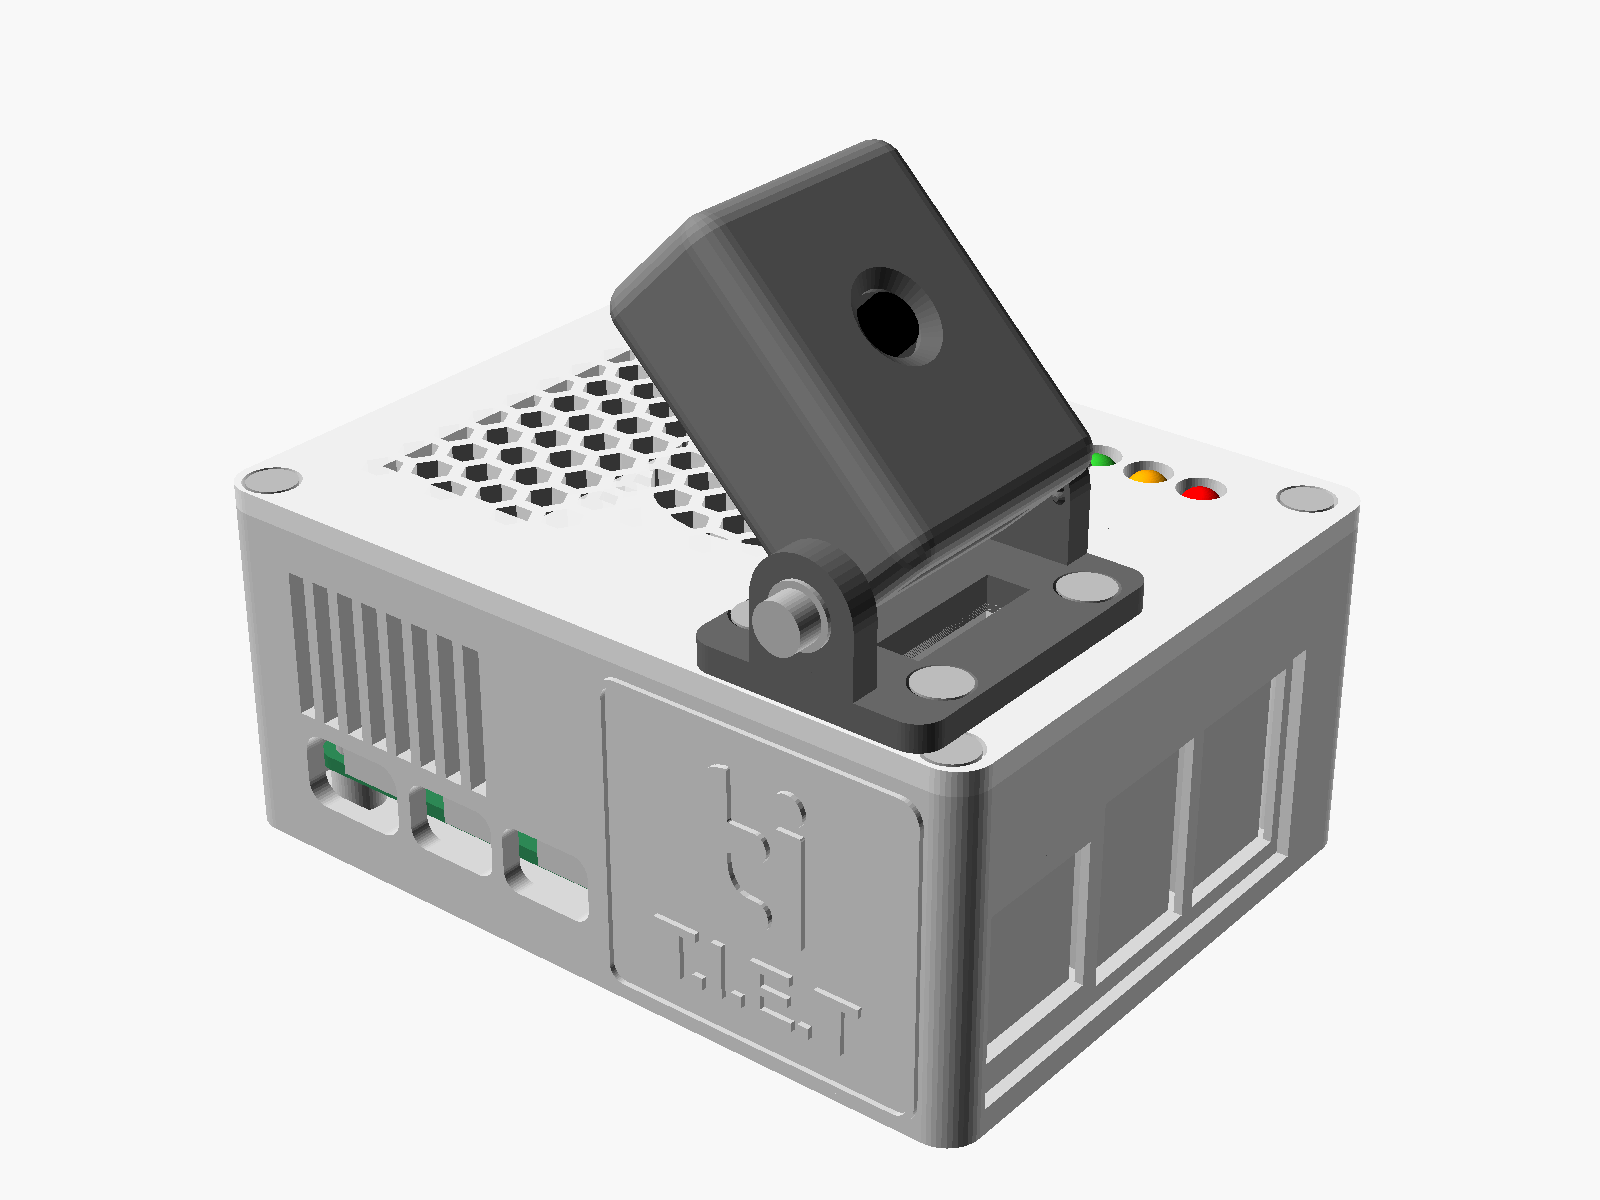
\includegraphics[width=0.32\textwidth]{figures/renders/1_assembled.png}\hfill
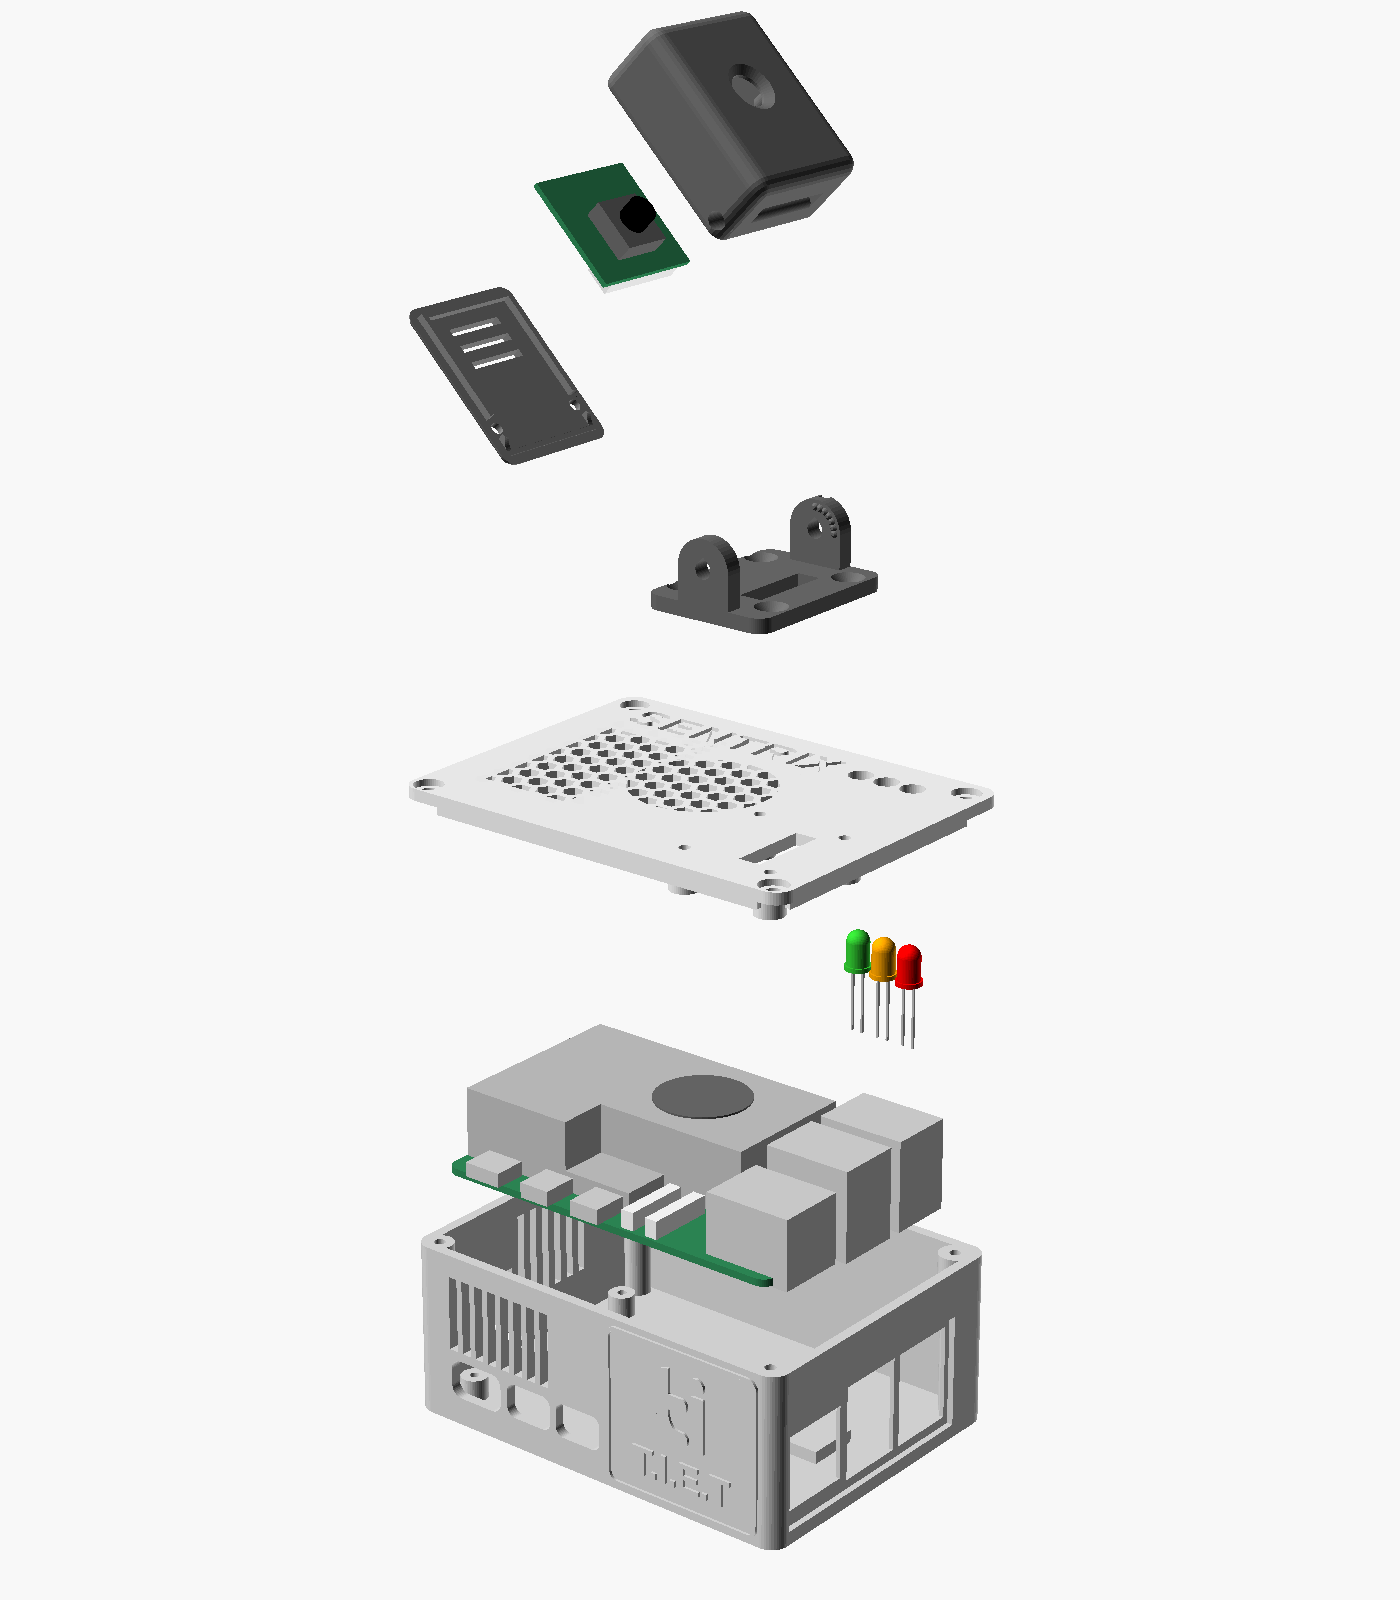
\includegraphics[width=0.32\textwidth]{figures/renders/2_exploded.png}\hfill
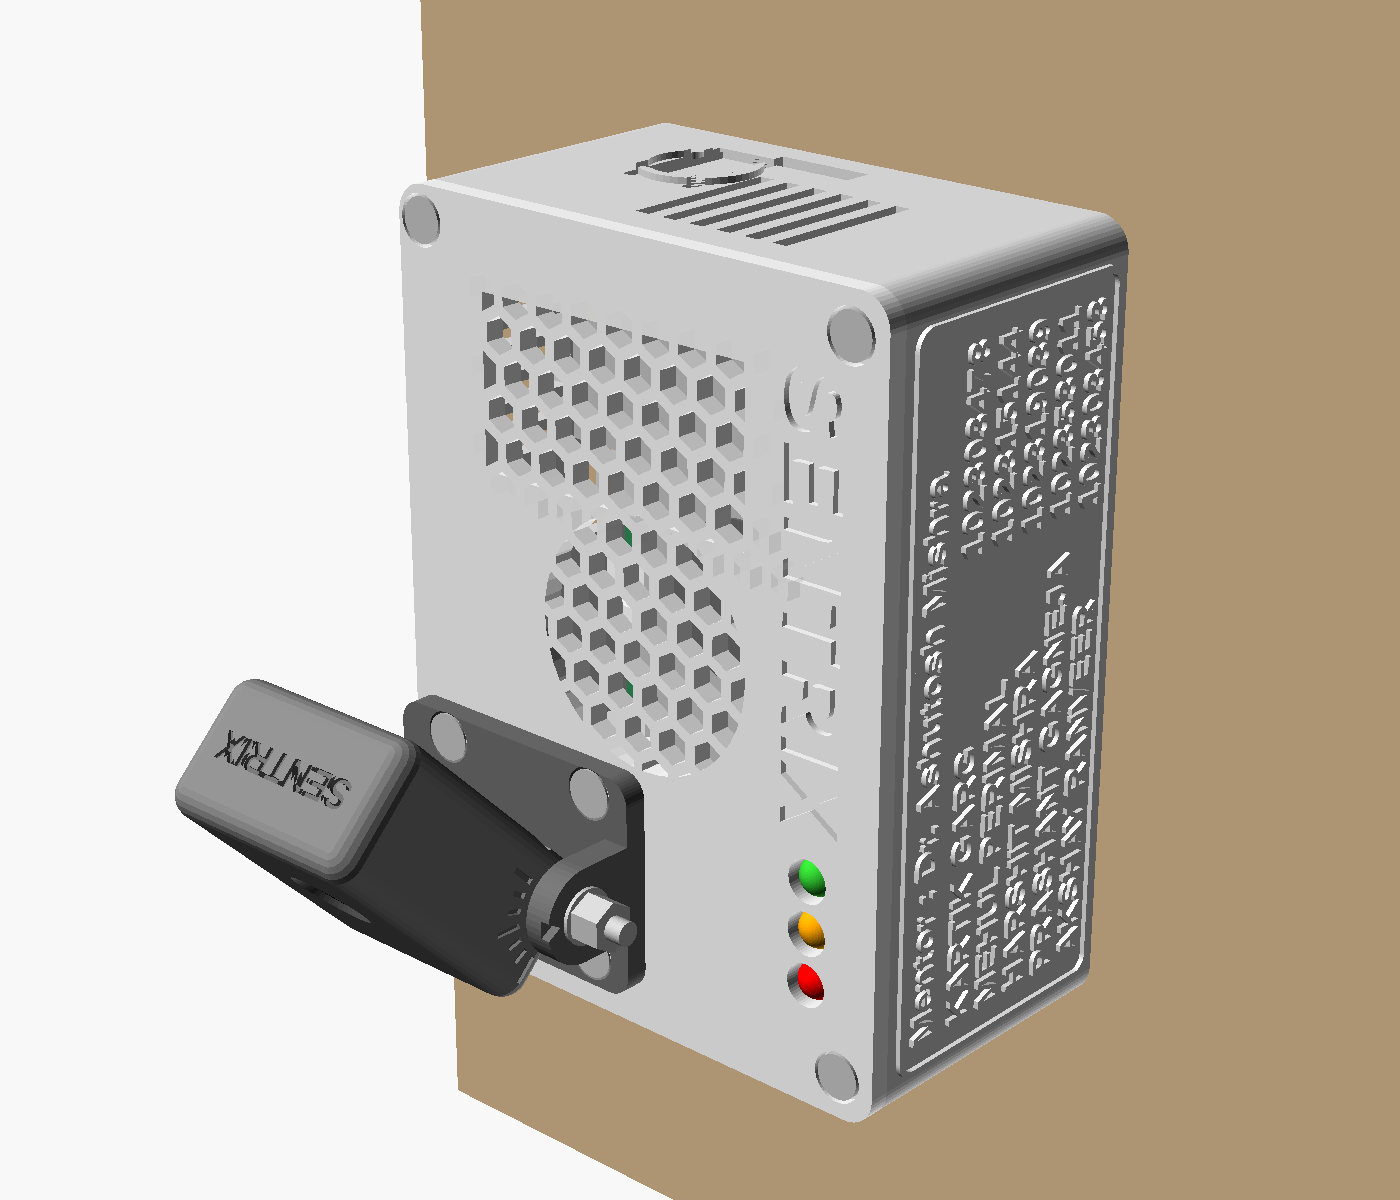
\includegraphics[width=0.32\textwidth]{figures/renders/9_wall_mounted.png}
\caption{Enclosure revision F: assembled, exploded, and wall-mounted with the camera end down}
\label{fig:enclosure}
\end{figure}
